%% Elsevier / Information and Software Technology draft.
%% Template source: official Elsevier elsarticle package downloaded 2026-06-05.
\documentclass[preprint,12pt]{elsarticle}

\usepackage{amssymb}
\usepackage{amsmath}
\usepackage{booktabs}
\usepackage{array}
\usepackage{longtable}
\usepackage{tabularx}
\usepackage{xltabular}
\usepackage{makecell}
\usepackage{enumitem}
\usepackage[protrusion=true,expansion=false]{microtype}
\usepackage{xurl}
\usepackage{float}

\newcolumntype{Y}{>{\raggedright\arraybackslash}X}
\setlength{\emergencystretch}{3em}
\setlength{\parindent}{1em}
\AtBeginDocument{\setlength{\bibsep}{0pt plus 0.2ex}}
\let\paperbibliography\bibliography
\renewcommand{\bibliography}[1]{{\footnotesize\paperbibliography{#1}}}

%% Float placement: keep full-width tables near their first mention instead of
%% deferring tall floats to the end of the document.
\renewcommand{\topfraction}{0.9}
\renewcommand{\bottomfraction}{0.8}
\renewcommand{\textfraction}{0.07}
\renewcommand{\floatpagefraction}{0.7}
\setcounter{topnumber}{3}
\setcounter{totalnumber}{5}

%% ---- Canonical NOETHER two-layer symbols (vendored from
%% P1-MetaPattern/shared/two_layer_canon.tex; single source of truth).
%% Term map: MR = metamorphic relation; MetaPattern = 元模式; MR family =
%% 蜕变关系族. Do not reintroduce "block" synonyms. ----
\providecommand{\AP}{\mathcal{A}_{P}}
\providecommand{\MM}{\mathbb{M}(\mathcal{A}_{P})}
\providecommand{\Grp}{G}
\providecommand{\Ord}{O_{\le}}
\providecommand{\Sadj}{T^{*}}
\providecommand{\Trev}{\mathcal{T}^{*}_{\mathrm{rev}}}
\providecommand{\Lim}{\mathcal{L}^{*}}
\providecommand{\minv}{m_{\mathrm{inv}}}
\providecommand{\mmono}{m_{\mathrm{mono}}}
\providecommand{\madj}{m_{\mathrm{adj}}}
\providecommand{\mrev}{m_{\mathrm{rev}}}
\providecommand{\mconv}{m_{\mathrm{conv}}}
%% L2 MR-family symbols (sans-serif f_{parent.child}), per two_layer_canon.tex.
\providecommand{\fIeqv}{\mathsf{f}_{\mathrm{inv}.\mathrm{eqv}}}
\providecommand{\fIcon}{\mathsf{f}_{\mathrm{inv}.\mathrm{con}}}
\providecommand{\fAself}{\mathsf{f}_{\mathrm{adj}.\mathrm{self}}}
\providecommand{\fAdual}{\mathsf{f}_{\mathrm{adj}.\mathrm{dual}}}
\providecommand{\fRtraj}{\mathsf{f}_{\mathrm{rev}.\mathrm{traj}}}
\providecommand{\fMstat}{\mathsf{f}_{\mathrm{mono}.\mathrm{stat}}}
\providecommand{\fMshape}{\mathsf{f}_{\mathrm{mono}.\mathrm{shape}}}
\providecommand{\fClim}{\mathsf{f}_{\mathrm{conv}.\mathrm{lim}}}
\providecommand{\fCrate}{\mathsf{f}_{\mathrm{conv}.\mathrm{rate}}}
\providecommand{\fCrepr}{\mathsf{f}_{\mathrm{conv}.\mathrm{repr}}}
\providecommand{\Translate}{\textsc{Translate}}

\journal{Information and Software Technology}

\begin{document}

\begin{frontmatter}

\title{Numerical-Decidability-Gated Metamorphic Testing for Scientific Machine Learning Surrogates}

\author[inst1,inst2,inst3]{Meng Li\corref{cor1}}
\ead{mlemon@usc.edu.cn}
\author[inst1,inst2,inst3]{Xiaohua Yang}
\ead{xiaohua1963@foxmail.com}
\author[inst1,inst2,inst3]{Jie Liu}
\ead{jieliu@usc.edu.cn}
\author[inst1,inst2,inst3]{Shiyu Yan}
\ead{yanshiyu@usc.edu.cn}
\cortext[cor1]{Corresponding author: Meng Li.}
\affiliation[inst1]{organization={School of Computing, University of South China},
  city={Hengyang}, postcode={421001}, country={China}}
\affiliation[inst2]{organization={Hunan Engineering Research Center of Software Evaluation and Testing for Intellectual Equipment},
  city={Hengyang}, postcode={421001}, country={China}}
\affiliation[inst3]{organization={CNNC Key Laboratory on High Trusted Computing},
  city={Hengyang}, postcode={421001}, country={China}}

\begin{abstract}
Scientific machine-learning (SciML) surrogates are hard to test because exact
outputs are unavailable for transformed inputs. Metamorphic testing can
turn physical relations into oracle-free tests, but a candidate relation is not
automatically an interpretable verdict: a failure may reflect a surrogate
inconsistency, an invalid relation application, or a numerical artifact of the
measurement operator. This article treats numerical decidability as an
admissibility condition for SciML metamorphic testing. The resulting predicate
checks physical basis, transformation preconditions, representation mapping,
and whether the verdict tolerance dominates the operator's intrinsic floor. It
is implemented through metamorphic-relation (MR) records, executable checks, typed verdicts,
and a fail-closed ledger. The numerical component is a discrete-divergence
floor bound instantiated on the cylinder-flow mesh, with a second topology
used as bounded stability evidence. The gate changes verdicts rather than only annotating
them: it defers absolute conservation when the floor dominates, rejects an
inadmissible airfoil continuity relation on physical-basis grounds, and keeps
node permutation as an implementation sanity check. Bounded MeshGraphNets,
PointMLP, physics-informed neural-network (PINN), Fourier-neural-operator (FNO),
airfoil, and cross-program executions show that detector
coverage follows the admitted relation set. The evidence supports an auditable
admissibility workflow for relation-indexed SciML verification and validation in the studied settings,
not general SciML reliability.
\end{abstract}

\begin{highlights}
\item Numerical decidability gates surrogate metamorphic-test verdicts.
\item Operator-floor bounds decide when divergence checks are measurable.
\item Relation records, verdicts, and ledgers make admissibility auditable.
\item Bounded executions show coverage follows the admitted relation set.
\item Results support complementarity, not baseline superiority.
\end{highlights}

\begin{keyword}
Metamorphic testing \sep oracle problem \sep scientific machine learning \sep software testing \sep verification and validation
\end{keyword}

\end{frontmatter}

\section{Introduction}
\label{sec:introduction}

SciML surrogates are now used as software components for approximating expensive simulations \citep{raissi2019pinn,karniadakis2021piml,li2021fno}. Mesh-based neural simulators such as MeshGraphNets (MGN) predict physical fields on irregular meshes \citep{pfaff2021meshgraphnets}, but they also inherit a classical testing difficulty: for many candidate inputs there is no cheap exact output against which the program can be checked, the test oracle problem \citep{barr2015oracle}. Held-out rollout error is therefore necessary, but it does not by itself tell a tester whether the software respects relations that should hold under physically meaningful transformations.

Metamorphic testing (MT) addresses the oracle problem by checking relations among multiple executions rather than a single expected output \citep{chen1998metamorphic,segura2016survey}. Conservation laws, symmetry relations, nondimensional similarity, and continuity conditions can all suggest candidate MRs for scientific software \citep{kanewala2019scientific,lin2020exploratory,olsen2019simulation}. The testing problem considered here begins after such candidates have been proposed. A physics-derived relation is not automatically a valid software test: mirror symmetry may depend on geometry and boundary labels; a divergence relation may depend on a discrete operator, mesh weights, and boundary treatment; a transformed case may leave the relation's domain before it reveals any system-under-test (SUT) inconsistency.

For SciML surrogate software, this creates an oracle-free verification-and-validation (V\&V) interpretability problem: when an MR check fails, the tester must ask whether the SUT violated a genuine relation, the relation was applied outside its validity conditions, the output mapping was incompatible with the software representation, or the scoring operator could not resolve the claimed effect. Treating all such outcomes as ordinary pass/fail MT verdicts makes the evidence hard to audit and easy to overclaim.

Here, numerical decidability is an admissibility condition for SciML MR use: before a candidate relation can serve as an oracle-free test, its verdict must be resolvable for the deployed discretization and measurement operator. The approach builds on MT and complements residual, uncertainty, accuracy, and trust-region diagnostics. It treats numerical decidability as a gate on relation admissibility, implements the gate through relation records, executable checks, and typed verdicts, and reports how the gate changes testing outcomes. A downgraded or rejected relation can still be reported as out-of-distribution (OOD) stress evidence; it is just not licensed as a SUT fault verdict. Physical knowledge, expert reasoning, large language model (LLM)-assisted candidate lists, and the NOETHER two-layer structure of MetaPatterns and MR families \citep{zhao2026noether} may suggest candidate relations; the gate decides which candidates become executable SciML V\&V checks.

Two principles organize the method. First, an MR is \emph{admissible} only when its validity conditions hold for the SUT and the verdict is numerically decidable: the tolerance must dominate the intrinsic floor of the measuring operator (machine precision, a mapping floor, or a discretization floor, by relation type). Second, relation-level verdicts are interpreted along two axes, relation-violation and domain-violation magnitude, separating SUT inconsistency from out-of-relation-domain application, numerical-floor deferral, and inconclusive evidence. We refer to the resulting framework as numerical-decidability-gated, relation-indexed SciML V\&V. The main empirical setting is MeshGraphNets-family cylinder flow, with the same admissibility predicate additionally exercised on a second computational fluid dynamics (CFD) task and additional partial differential equation (PDE) families; these are bounded case studies, not cross-domain reliability estimates.

Contributions are fourfold:
\begin{itemize}[leftmargin=*]
\item The numerical-decidability admissibility gate is defined for SciML MR testing: a relation-level verdict is admissible only when its tolerance dominates the intrinsic numerical floor of the measurement operator. For the deployed cylinder-flow divergence check, this criterion is instantiated by a discrete-divergence floor bound, a measured floor matched by a closed-form predictor, a dominating a-priori upper bound, and a second-topology stability check (Sec.~\ref{subsec:operator-floor-sweep}). The detailed statement is kept with the operator-floor experiment, where the operator class and mesh assumptions are defined before use.

\item The criterion is implemented as auditable executable checks. Each admitted relation is represented as a relation record and executable check that records the transformation, mapping, metric, tolerance, exclusion rule, and ledger fields needed for inspection.

\item The typed domain-inadmissibility verdict separates relation violation from domain violation, instantiating for physics-governed SciML the constraint-architecture pattern behind bug-versus-inapplicability reasoning \citep{duqueTorres2023bugornot,duqueTorres2023completePipeline} and MetaTrimmer \citep{duqueTorres2023metaTrimmer}.

\item The case studies evaluate what the criterion changes beyond rollout accuracy, generic MR generation, and LLM-assisted MR candidate elicitation, drawing primarily on MeshGraphNets cylinder-flow runs with supporting airfoil, PINN, FNO, and cross-program checks. The admitted MR set is also used as a seeded-fault diagnostic stress test for interpreting fault-detection boundaries and blind spots in the studied settings.
\end{itemize}

Section~\ref{sec:related} positions the work against oracle-free testing, physics-based MT, and SciML diagnostics. Section~\ref{sec:method} defines the gate, relation record, executable check, and verdicts. Section~\ref{sec:empirical-design} states the research questions, subjects, metrics, baselines, and analysis plan. Section~\ref{sec:results} reports the empirical evidence and claim boundaries, followed by threats to validity, future work, and conclusions.

\section{Related Work}
\label{sec:related}

\subsection{SciML surrogates, oracle-free testing, and MR candidate sources}
\label{subsec:mesh-simulation}
\label{subsec:mt-oracle}
\label{subsec:mr-identification}

Mesh-based neural simulators learn dynamics on graph or mesh representations of physical systems. MeshGraphNets encodes mesh nodes and edges, propagates information by message passing, and predicts future physical fields through autoregressive rollout \citep{pfaff2021meshgraphnets}. Here these models are treated as software SUTs. The testing question is whether a rollout is accurate on held-out trajectories and whether the SUT preserves declared relations under controlled transformations and explicit tolerances.

MT addresses programs lacking a per-input oracle \citep{chen1998metamorphic,segura2016survey,chen2018mtSurvey}. Rather than checking each output against an expected value, MT checks a relation among source and follow-up executions. This framing has been applied to scientific software, PDE programs, simulations, and machine-learning (ML) systems \citep{chen2002pde,chen2011ml,kanewala2019scientific,olsen2019simulation}, including recent applications to tabular ML such as credit scoring \citep{ying2025}. For SciML surrogates, however, an MR is not merely an input perturbation: its validity depends on governing equations, boundary conditions, mesh representation, output mapping, and numerical tolerance. This makes MR admissibility part of the oracle construction problem itself.

Testing scientific software without a reliable oracle is a long-standing problem, and metamorphic testing is the most developed response in the surveyed literature \citep{kanewalaBieman2014slr}. MRs can be elicited from monotonicity, conservation, scaling, and domain-specific expectations \citep{kanewala2019scientific,lin2020exploratory,olsen2019simulation,raunak2021continuum}. Predictive MR identification has been pursued with graph-kernel learning over scientific source code \citep{kanewala2016graphkernel}, by separating input and output patterns and by image-based output-pattern recognition for numerical solver codes \citep{wang2022mridentification,fu2021burnup}, and with large language models that discover metamorphic-relation variables for scientific software \citep{tsigkanos2023}. Symmetry-based MRs paired with statistical violation criteria have also been applied to deep trajectory predictors \citep{spieker2024trajectory,spieker2025multimodal}. Data-driven search can discover candidate transformations in complex physical software \citep{hiremath2021ocean}, and design assumptions can be encoded as MRs for cyber-physical-system (CPS) testing under control--plant invariants \citep{mandrioli2025cps}.

Separate work has made MR specification and applicability more explicit. General MT tooling has explored machine-readable MR representations, constraint definition, test-data-driven MR selection, and general MR specification languages \citep{duqueTorres2023completePipeline,duqueTorres2024selecting,sun2026ccml}. These systems strengthen MR engineering in the large, but they do not by themselves decide whether a physics-derived relation is numerically measurable, in-domain for a transformed CFD case, or interpretable as a SciML V\&V verdict.

These approaches can supply candidate sources, but candidate identification is not admissible SciML test construction. MR identification, including our own prior physics-derived MR construction for numerical solver and nuclear-power software \citep{li2022nuclearmr,wang2022mridentification}, is established work; the candidate MRs are treated as inputs, and the contribution is the admissibility gate rather than a new identification method. Fault-oriented MR work ranks relations by observed detection power \citep{srinivasan2022prioritization,saha2019faultdetection}; the admitted relation set is used later to interpret bounded coverage and blind spots, as a consequence of admissibility rather than as the primary novelty.

\subsection{Physics-based MT, tolerance, and applicability}
\label{subsec:physics-mt}

Three contemporary strands are closest to the present work. Yang and Chui \citep{yang2021hydromt} and Reichert et al.~\citep{reichert2024hess} applied physics-derived MRs to hydrologic ML or conceptual models, showing that learned-model accuracy and relation consistency can diverge and that calibration or forcing regimes affect interpretation. Eniser et al.~\citep{eniser2022relaxations} introduced \emph{relaxations}, numerical tolerances embedded in MR oracles, for stochastic reinforcement-learning (RL) policy testing. Duque-Torres et al.~\citep{duqueTorres2023bugornot,duqueTorres2023completePipeline,duqueTorres2024selecting} and MetaTrimmer \citep{duqueTorres2023metaTrimmer} address bug-versus-inapplicability reasoning with explicit MR constraints and automated constraint derivation.

These ideas are combined in a SciML-specific V\&V workflow. From physics-based MR testing it takes relation-level checks; from relaxations it takes the need for calibrated tolerances; from violation-attribution work it takes the need to avoid treating inapplicability as a SUT failure. What none of these strands supplies is the central condition used here: admissibility made contingent on numerical decidability. Existing work may constrain when an MR applies or relax an oracle tolerance; this work adds a prior admissibility requirement that the tolerance dominate the measuring operator's intrinsic numerical floor before any SUT-failure verdict is licensed.

The closest prior work covers complementary parts of the problem rather than the whole candidate-to-verdict path. Reichert et al.~\citep{reichert2024hess} show that physics-derived MRs can reveal consistency issues in learned hydrologic surrogates, but the filtering remains informal and does not define a reusable admissibility-to-verdict workflow. Eniser et al.~\citep{eniser2022relaxations} introduce relaxed MR oracles, but their tolerance is not tied to the measuring operator's intrinsic numerical floor. Duque-Torres et al.~\citep{duqueTorres2023bugornot,duqueTorres2023completePipeline,duqueTorres2024selecting}, MetaTrimmer~\citep{duqueTorres2023metaTrimmer}, and related MR-specification tools~\citep{sun2026ccml} make applicability constraints explicit, but they do not provide SciML-specific physical, geometric, boundary-condition, and operator-floor verdict types. The gap addressed here is the combination of an explicit admissibility predicate, operator-floor numerical decidability, executable relation records, and typed verdicts for physics-governed SciML surrogate software; Table~A2 in the supplementary evidence appendix gives the full closest-prior capability matrix.

\subsection{SciML diagnostics and positioning}
\label{subsec:sciml-vv}
\label{subsec:hybrid-trust}
\label{subsec:new-not-new}

SciML reliability research has developed complementary tools: physics residuals, uncertainty quantification (UQ), conformal prediction, certified error bounds, and failure-mode analysis \citep{raissi2019pinn,karniadakis2021piml,li2021fno,krishnapriyan2021failure,gopakumar2025calibrated}. PINN training can exhibit gradient-flow pathologies that bias trained models away from the governing residual \citep{wang2021gradflow,krishnapriyan2021failure}, sharpening the need for checks that do not assume a converged surrogate. These diagnostics are not competitors to MT. A residual, equivariance error, or uncertainty score becomes an executable MR only when paired with a source case, follow-up transformation, tolerance rule, exclusion rule, and verdict interpretation. The proposed workflow uses such diagnostics as possible measurements inside a multi-execution oracle-free check.

Hybrid ML-solver frameworks use residual thresholds or error estimates to decide when a learned component should be trusted \citep{baral2025xrepit,wang2025deeponetfe}. Such systems operationalize runtime trust regions, whereas the proposed workflow acts offline, applying physically derived transformations before deployment to estimate where relation violations occur.

The distinction from residual- and uncertainty-based trust estimation is deliberate. UQ, conformal prediction, residual-threshold trust regions, and physical-consistency diagnostics that score a physically derived residual on observed outputs \citep{najafi2026} locate unreliable behavior from observed inputs. The present method acts in relation space: it applies a controlled transformation and reports which necessary relation breaks under it, indexed by that transformation. The claim is complementarity, not superiority: relation-indexed evidence answers a different question from scalar accuracy, residual magnitude, or uncertainty.

The preceding subsections reviewed metamorphic testing, MR identification, scientific-software MT, residual and uncertainty diagnostics, LLM-assisted candidate generation, and the NOETHER two-layer structure of MetaPatterns and MR families as sources of testing ideas. The contribution here is narrower: SciML MR use should be treated as an admissibility and executable-check problem. A candidate relation becomes a useful oracle-free V\&V check only after its physical basis, transformation preconditions, output mapping, tolerance, exclusion rule, executable check, and relation-level verdict are recorded. Recent work derives or refines domain-specific MRs for scientific programs directly from their numerical models \citep{yan2024elliptic,stevens2025mars}; the wedge here is the learned surrogate evaluated out of distribution and the requirement that a relation's tolerance dominate the measuring operator's numerical floor, rather than testing a numerical solver against derived relations. The missing combination is thus an admissibility-gated, executable, and auditable workflow for physics-governed SciML surrogate software.

\section{Admissibility-Gated MR Workflow}
\label{sec:method}

\subsection{Overview}
\label{subsec:method-overview}

The method turns a physics-derived candidate relation into an auditable V\&V check only after three steps are made explicit: admissibility, executable checking, and verdict interpretation. These three design roles are evaluated by the research questions introduced in Section~\ref{subsec:rqs}. Figure~\ref{fig:workflow} summarizes the workflow. Candidate generation is deliberately separated from validity judgment: expert reasoning, physical laws, the NOETHER two-layer structure of MetaPatterns and MR families, and LLM-assisted lists may propose relations, but none certifies a relation as valid for a specific SUT.

\textbf{Definitions.} Let \(r=(b,T,M,m,\tau,P)\) denote a candidate relation. Here \(b\) is the physical or software basis, \(T\) is the source-to-follow-up transformation, \(M\) maps follow-up outputs back into the comparison space, \(m\) is the metric, \(\tau\) is the verdict tolerance, and \(P\) is the set of source and follow-up preconditions. For a SUT \(s\) and source case \(x\), the admissibility gate returns
\[
G(r,s,x)\in\{\mathrm{admit},\mathrm{reject},\mathrm{stress},\mathrm{defer}\}.
\]
If the relation is admitted, or retained only as stress evidence, the executable check returns \(E(r,s,x)=(y,y',z)\), where \(y\) and \(y'\) are the source and follow-up outputs and \(z\) is the measured relation evidence. A verdict map \(V(G,z)\) then assigns the typed verdict. Only an admitted relation with an in-domain fail verdict may support a SUT-inconsistency claim; rejected, stress-only, deferred, or inconclusive outcomes remain evidence about the relation, the domain, or the measurement setup.

\textbf{Terminology and verdict types.} A verdict is read on two axes, relation-violation and domain-violation magnitude (detailed in Sec.~\ref{subsec:verdicts}). A candidate relation is accordingly \emph{admitted} (a large in-domain violation reads as SUT inconsistency), \emph{rejected} on physical grounds, \emph{deferred} when no tolerance dominates the operator floor, \emph{out-of-relation-domain}, or \emph{inconclusive}. Four MR families recur in the case studies: node-permutation equivariance, mirror-y reflection symmetry, discrete-divergence continuity/conservation, and exact mirror-y on a constructed symmetric mesh. As a running example, a mirror-y candidate is first checked against geometry and boundary labels; on an asymmetric mesh it becomes OOD stress rather than a fault oracle, while on a constructed symmetric mesh it remains an admitted equivariance test.

\begin{figure}[!htbp]
\centering
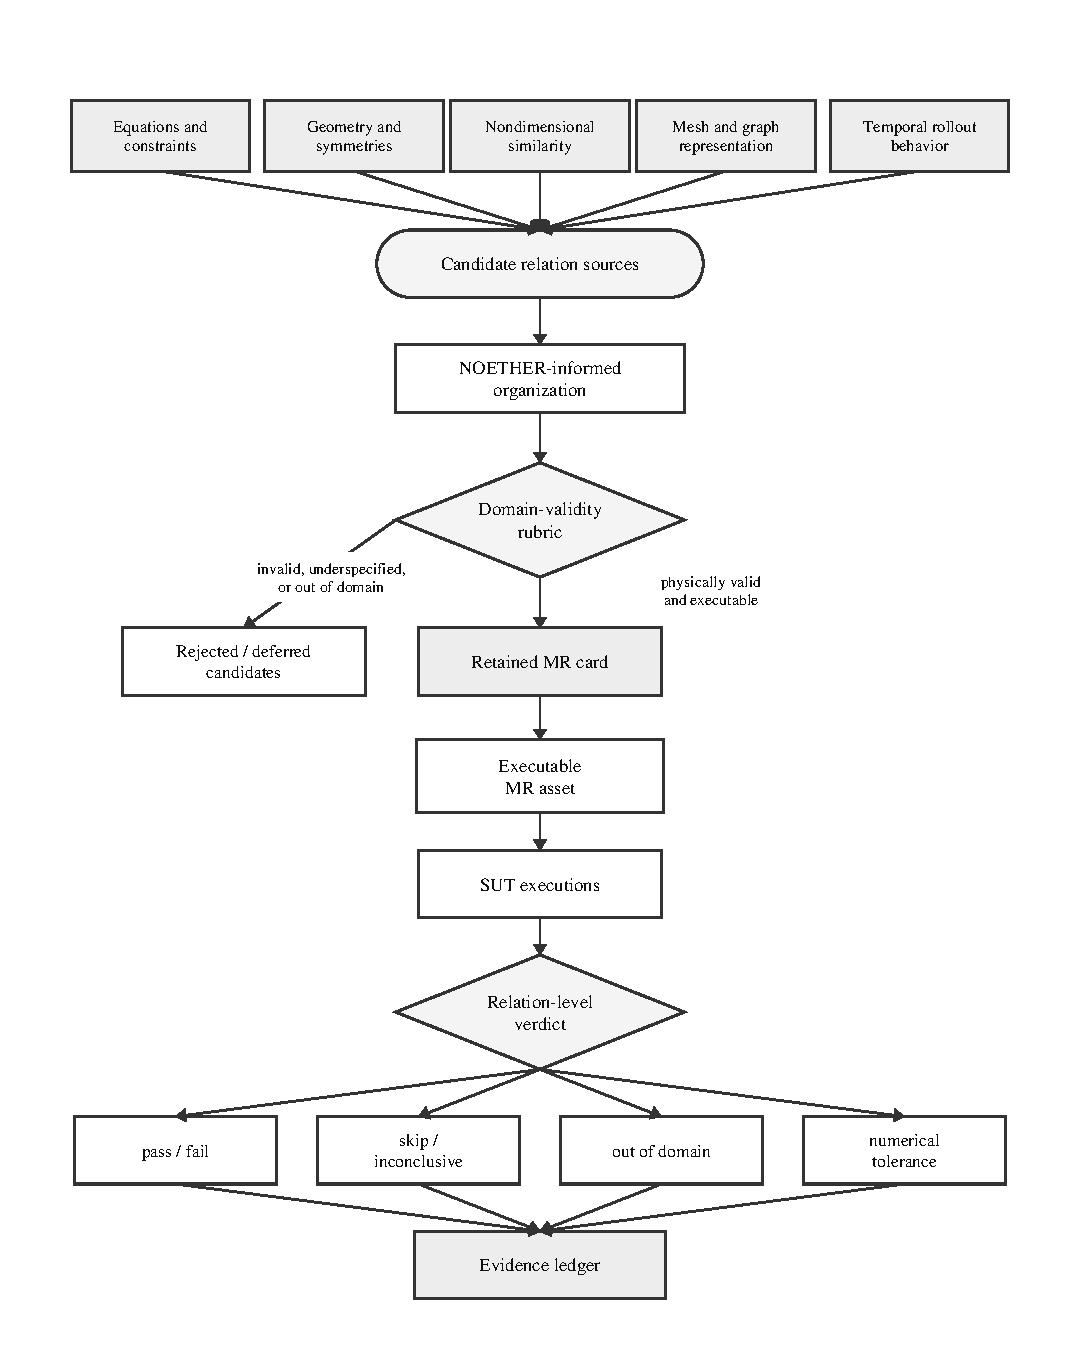
\includegraphics[width=0.95\linewidth]{figures/fig_1_validity_gated_workflow.pdf}
\caption{Admissibility-gated V\&V workflow.}
\label{fig:workflow}
\end{figure}

\subsection{Candidate relation sources and organization}
\label{subsec:candidate-sources}

Two prior MR-identification results are used here rather than redefined. The four-layer classification of scientific-computing MRs \citep{yang2020hierarchical} asks where relations come from: physical, computational, code, or data layers. Its physical, computational, and code layers can yield real MRs when the corresponding semantic constraint is established. NOETHER \citep{zhao2026noether}, a same-author preprint, asks a different question: what structural form an MR can take when it is induced by algebraic properties of the equation or program operator. It proposes a two-layer structure: MetaPatterns identify the algebraic source pattern, and MR families instantiate those patterns as transformation-and-comparison templates. Together, these prior results source and organize candidate relations; NOETHER is used only as an optional scaffold for generating and naming likely MR candidates. The central decision point is therefore not candidate discovery itself but the admissibility gate of Section~\ref{subsec:admissibility-gate}, which decides whether any candidate becomes an admissible MR for a specific SUT.

\emph{Layer~1 (MetaPattern).} A \emph{MetaPattern} is the equivalence class of MRs generated, through \Translate, from one minimal algebraic structure of the program-induced operator algebra $\AP$. The five MetaPatterns are generated by a group action ($\Grp$), partial order ($\Ord$), self-adjoint operator ($\Sadj$), time-reversal involution ($\Trev$), or parametrized limit ($\Lim$); their set is $\MM$. Conservation is therefore the group-action member $\minv$.

\emph{Layer~2 (MR family).} An \emph{MR family} instantiates one MetaPattern under a fixed transformation template and mode. Families use the form $\mathsf{f}_{\mathrm{parent}.\mathrm{child}}$; legacy letters a--j remain cross-reference anchors. The map is one-to-many: $\Grp \to \{\fIeqv, \fIcon\}$, $\Sadj \to \{\fAself, \fAdual\}$, $\Trev \to \{\fRtraj\}$, $\Ord \to \{\fMstat, \fMshape\}$, and $\Lim \to \{\fClim, \fCrate, \fCrepr\}$.

For the cylinder-flow surrogates studied here, the instantiated families are $\fIeqv$ (equivariance, a), mirror-y reflection; $\fIcon$ (conservation, b), discrete-divergence continuity and, on the airfoil task, compressible mass balance; $\fCrepr$ (representation-invariance, j), node-permutation and encoding contracts; and $\fClim$ and $\fCrate$ (convergence, accuracy-order, h--i), the operator-floor mesh-refinement relation. The $\fMstat$ (static-order, f) Reynolds--Strouhal monotonicity is a candidate not exercised here, $\fRtraj$ (trajectory-reversal, e) is empty by construction for viscous dissipative flow, and the self-adjoint families $\fAself$ and $\fAdual$ (c--d) appear only in the cross-family PINN and FNO extensions. The same relation may be admissible as one family yet inadmissible once instantiated for a given SUT: mirror symmetry holds on a symmetric domain but not on an asymmetric mesh with incompatible boundary labels, and conservation is a physical expectation but not an executable verdict when the discrete measuring operator has an unresolved floor. The admissibility gate records where each relation survives.

\subsection{Admissibility gate}
\label{subsec:admissibility-gate}

A candidate relation is an \emph{admissible MR} only when four conditions hold together. First, it must have a physical or software basis. Second, its transformation preconditions must hold for the source and follow-up cases. Third, boundary conditions and output mappings must remain compatible after transformation. Fourth, the verdict must be numerically decidable: the tolerance must dominate the intrinsic error floor of the measuring operator. None of these conditions is optional. Table~\ref{tab:admissibility-gate} records the gate, the relation-record fields, and the verdict semantics.

\begin{table}[!htbp]
\centering
\caption{Admissibility gate and verdict semantics.}
\label{tab:admissibility-gate}
\footnotesize
\renewcommand{\arraystretch}{0.92}
\setlength{\tabcolsep}{3pt}
\begin{tabularx}{\textwidth}{@{}>{\raggedright\arraybackslash}p{0.18\textwidth}>{\raggedright\arraybackslash}p{0.31\textwidth}>{\raggedright\arraybackslash}p{0.29\textwidth}Y@{}}
\toprule
\textbf{Method element} & \textbf{Required record} & \textbf{Allowed interpretation} & \textbf{Design role} \\
\midrule
Basis & Equation, boundary condition, nondimensional law, representation property, numerical assumption, or implementation contract & Relation may be considered only for SUTs where this basis applies & Gate \\
Preconditions & Source-case constraints, follow-up transformation, preserved quantities, and exclusion rule & Missing preconditions produce skip or out-of-relation-domain, not SUT failure & Gate \\
Mapping compatibility & Boundary-label compatibility and output mapping from follow-up output back to source coordinates/fields & Incompatible mapping rejects or downgrades the candidate & Gate \\
Numerical decidability & Metric, tolerance, tolerance provenance, and measurement-floor evidence & A verdict is meaningful only when tolerance dominates the operator floor & Gate \\
Relation record & Identifier, source category, transformation, mapping, metric, tolerance, exclusions, expected verdicts, and schema & The admitted relation becomes a reusable executable check & Check \\
Ledger & Source/follow-up run ids, metric outputs, floor evidence, exclusions, logs, and verdict & The reported claim is auditable from evidence rather than prose alone & Ledger \\
Verdict semantics & Pass, fail, skip, out-of-relation-domain, numerical-tolerance issue, or inconclusive & Only fail inside the valid domain may be read as SUT inconsistency & Verdict \\
\bottomrule
\end{tabularx}
\end{table}

The gate produces four design-time decisions: admit as an executable MR; downgrade to OOD-stress when the relation is physically informative but outside its exact domain; reject when basis, preconditions, or mapping fail; or defer when missing numerical evidence prevents a verdict. For example, node permutation can be admitted as a representation MR when the adapter and inverse mapping are deterministic; mirror-y is conditional on compatible geometry, boundary labels, and vector-component mapping; absolute discrete divergence is deferred when the reference field and measuring operator floor cannot support an absolute verdict.

\subsection{Relation record and executable check format}
\label{subsec:relation-record}

A retained MR is represented as a relation record containing the fields listed in Table~\ref{tab:admissibility-gate} plus interpretation limits. The record derives from the five core concepts; the executable check operationalizes it.

Each executable check includes transformation code, runner configuration, metric computation, verdict logic, and evidence recording. The ledger is part of the method rather than only replication packaging: every relation-level claim must be traceable to the source run, follow-up run, mapping, metric output, floor evidence, exclusion decision, and verdict.

\subsection{Relation-level verdicts}
\label{subsec:verdicts}

An MR execution can produce: \textbf{pass} (relation holds within tolerance); \textbf{fail} (violated within the valid relation domain); \textbf{skip} (required precondition missing); \textbf{out-of-relation-domain} (the transformed case is outside the relation domain); \textbf{numerical-tolerance issue} (the measured effect is dominated by threshold or resolution uncertainty); or \textbf{inconclusive} (insufficient artifact).

These verdicts form the two-dimensional space in Figure~\ref{fig:verdict-2d}. One axis is relation-violation magnitude, typically expressed as a violation-to-floor or violation-to-tolerance ratio. The other is domain-violation magnitude: how far the transformed case lies outside the relation's validity domain. Low domain violation with high relation violation is the region that may be read as SUT inconsistency; high domain violation is out-of-relation-domain; a violation inside the error floor is a numerical-tolerance issue. This decomposition defines the method's verdict-interpretation role, which is evaluated explicitly in Section~\ref{subsec:rqs}.

Here, the domain-violation coordinate is operationalized per relation from committed measurements. For mirror-y, $D = m/(m+1)$, where $m$ is the worst reflected-node placement error in median-edge-length units. The synthetic symmetric mesh scores $D \approx 0$, whereas the real asymmetric evaluation mesh scores $D = 0.51$. Other MR families use their own precondition measurements. These $D$ values denote structural placement within each relation's own validity domain: $D$ is a per-relation normalized coordinate, not a cross-relation calibrated metric, and the values cannot be averaged or ranked across MR families; read per relation, not as a calibrated boundary measurement. A cross-relation calibration would need to normalize each family by its own admissibility boundary, mapping every gate threshold to a common $D_{\mathrm{cal}} = 1$; that calibration is future work.

\begin{figure}[!htbp]
\centering
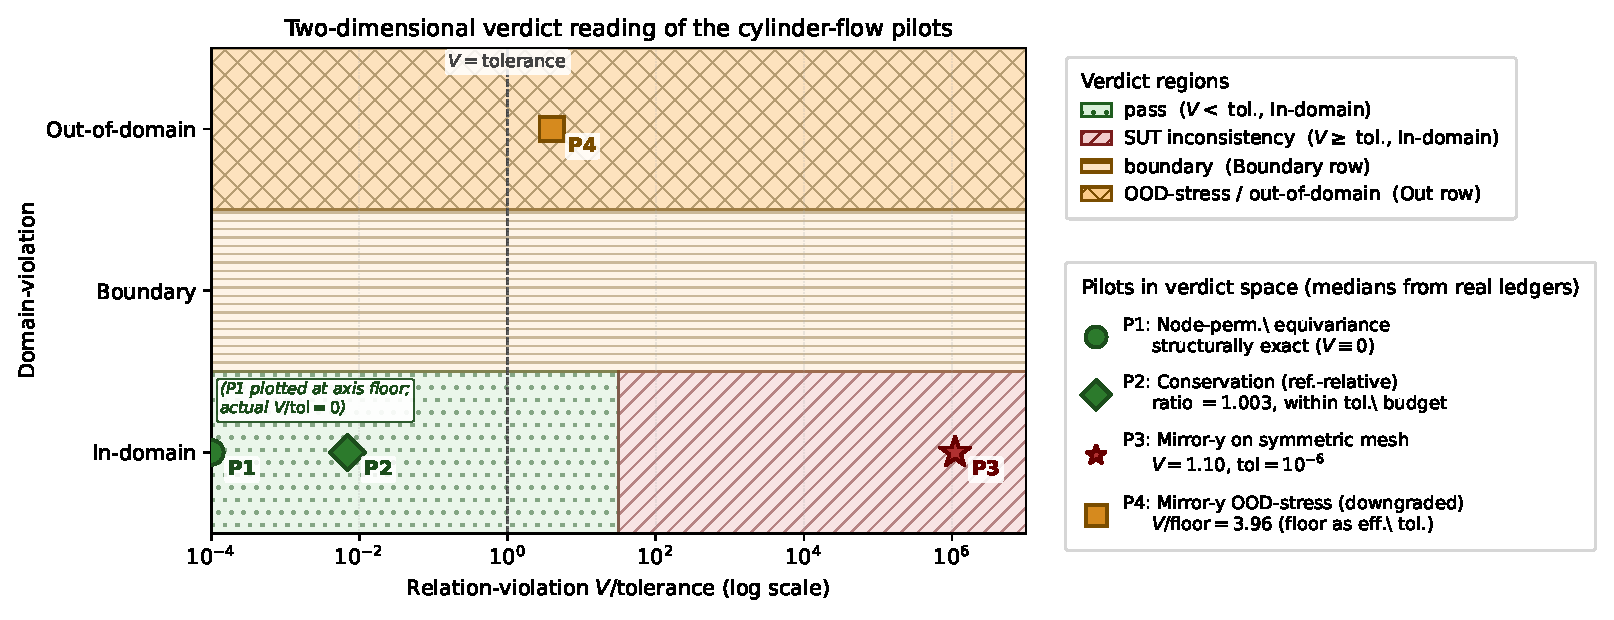
\includegraphics[width=0.98\linewidth]{figures/fig_3_verdict_2d.pdf}
\caption{Two-dimensional relation and domain verdict space.}
\label{fig:verdict-2d}
\end{figure}

Retained MRs are interpreted through their two-layer position (Sec.~\ref{subsec:candidate-sources}): a relation's MetaPattern and MR family fix which algebraic invariant it measures, and therefore which faults it can and cannot surface. This is an interpretation protocol, not a validated localization model; the seeded-fault results later are a bounded stress test of it.

\paragraph{Practitioner checklist and adoption boundary}
For a new SUT: (1) state the relation and source; (2) record source/follow-up preconditions; (3) check boundary labels and output mapping; (4) bound or calibrate the operator floor; (5) compare verdict tolerance with that floor; and (6) issue a typed verdict and ledger the run. The method does not remove domain expertise or automate MR discovery. Adoption costs are relation-specific physics review, mapping code, floor evidence, and bookkeeping; when any item is missing, the outcome is reject, defer, or OOD-stress, without a fault claim.

\section{Experimental Design}
\label{sec:empirical-design}

\subsection{Research questions}
\label{subsec:rqs}
\label{subsec:evaluation-logic}

The experimental design is organized around the following objective: to evaluate whether physics-derived MRs for SciML surrogate software can be transformed into auditable, executable, and interpretable oracle-free V\&V checks that distinguish genuine SUT inconsistency from relation invalidity and numerical measurement limits.

This objective is decomposed into four research questions:

\textbf{RQ1 -- Admissibility.} What validity conditions determine whether a physics-derived candidate MR is admissible as an oracle-free test for a specific SciML surrogate SUT?

\textbf{RQ2 -- Records and checks.} How can admissible MRs be represented as reusable relation records and executable checks with explicit transformations, mappings, metrics, tolerances, exclusions, and evidence records?

\textbf{RQ3 -- Verdict interpretation.} How can relation-level verdicts separate SUT inconsistency from out-of-relation-domain application, numerical tolerance limits, and inconclusive evidence?

\textbf{RQ4 -- Empirical utility.} In bounded SciML surrogate case studies, what evidence does the admissibility-gated workflow provide beyond rollout accuracy, generic MR generation, and LLM-assisted candidate elicitation?

\subsection{Experimental subjects}
\label{subsec:suts}

The subjects are selected for evidence roles rather than for statistical representativeness. A subject is included only when it contributes at least one design need: a primary end-to-end SciML surrogate setting with executable checks; a changed physical task or architecture that can falsify a checklist-only reading of the gate; a cross-family PDE/neural-operator setting that exercises the same admissibility predicate; or a bounded defect/coverage witness that ties MR responses to committed fault or true-fault-class evidence. The study does not select subjects by repository popularity, lines of code (LOC), or issue/changelog-mined defects; those criteria would require a separate real-defect study. The evidence below therefore supports bounded V\&V utility and coverage interpretation, not population-wide defect-detection effectiveness. Here, \(K\) is roster size. In the cylinder-flow roster, S0--S3 denote four baseline MeshGraphNets checkpoint configurations, and S4/S5 denote two same-domain wider/deeper MeshGraphNet variant configurations; together S0--S5 form the \(K=6\) roster.

In aggregate, the executable subject inventory comprises one primary CFD task, one second CFD task, same-task MGN variants, one PointMLP SUT, PhysicsNeMo executions, PINN and FNO rosters over two PDEs, one independent periodic-advection primary workflow, and five external central-processing-unit (CPU)-only SUT replays. The fault-evidence inventory comprises 10 canonical MGN mutants, two adversarial MGN mutants, 48 PINN/FNO output-level probes, a PointMLP 20-fault catalogue, and the external sibling's 70 witness rows and 20 true-fault-class rows. These counts are denominators for evidence scope; they are not sampling frames for a general defect-detection rate.

\begin{table}[!htbp]
\centering
\caption{Subject selection and evidence scope.}
\label{tab:subject-scope}
\scriptsize
\renewcommand{\arraystretch}{0.9}
\setlength{\tabcolsep}{3pt}
\begin{tabularx}{\linewidth}{@{}>{\raggedright\arraybackslash}p{0.20\linewidth}>{\raggedright\arraybackslash}p{0.45\linewidth}Y@{}}
\toprule
\textbf{Evidence block} & \textbf{Subjects and evidence role} & \textbf{Boundary} \\
\midrule
Cylinder-flow mesh surrogates & Primary executable workflow plus same-task implementation checks: MGN K=6 roster over three trajectories (S0--S3 baseline configurations plus S4/S5 wider/deeper variants), PointMLP, and PhysicsNeMo \texttt{MeshGraphNet}; seeded-fault stress uses 10 canonical MGN mutants, two adversarial mutants, and PointMLP 20-fault catalogue & Same task and bounded rosters; no real-defect rate or LOC-based representativeness \\
Airfoil mesh surrogate & Changed-physics gate discrimination on official DeepMind airfoil with PhysicsNeMo \texttt{MeshGraphNet}, K=6 checkpoints over 10 test trajectories & Typed inadmissibility evidence, not state-of-the-art airfoil accuracy or official-checkpoint evidence \\
PINN/FNO and periodic PDE workflows & Cross-family PINN/FNO Burgers/heat predicate checks plus independent periodic-advection primary workflow with six periodic-convolution SUTs and 60 relation cells per admitted MR & Synthetic/generated PDE evidence; not production CFD, real-defect, reliability, or broad neural-operator claims \\
External sibling programs & Minimum-MR-SubSet audit across seven program types plus five CPU-only end-to-end replays, including OpenMC and three SciML/PDE rows labeled \texttt{PASS\_WITNESS}, the sibling repository's tag for a passed witness replay & Read-only/sibling provenance; no new issue/changelog mining here \\
\bottomrule
\end{tabularx}
\end{table}

\emph{Primary evidence} comes from two bounded full-chain workflows. The first is a MeshGraphNets-family cylinder-flow case study: a trained checkpoint, its K=6 roster (S0--S3 plus S4/S5 as defined above), a PointMLP coordinate network, and NVIDIA PhysicsNeMo \texttt{MeshGraphNet} on official DeepMind cylinder\_flow TensorFlow Record (TFRecord) files. The second is an independent synthetic periodic-advection workflow: six NumPy-trained periodic-convolution SUTs, ten held-out fields per SUT, two admitted MRs, and one rejected candidate. In both workflows, the primary unit is a relation-level cell: relation record, SUT/checkpoint, source case, transformed follow-up case, metric, and verdict.

\emph{Supporting evidence} checks whether the same admissibility predicate applies outside the primary mesh-surrogate setting: airfoil gate discrimination, a fifteen-seed PINN roster (K=15), and trained two-dimensional FNO (FNO-2D) checkpoints over two-dimensional Burgers and heat data. The FNO admissibility roster is admitted on 15/15 per PDE for its periodic candidate set; the executable FNO workflow below is the smaller trained-checkpoint verdict run, not a broad neural-operator rate.

\emph{Secondary evidence} includes LLM-simulated expert MR design, generic MR-generation scope contrasts, LLM-assisted candidate generation, rollout-accuracy diagnostics, and external witness reruns from the read-only Minimum-MR-SubSet repository. \emph{Secondary baseline and external-scope audit} results are scope contrasts: LLM baselines are secondary exploratory scope contrasts, generic-MR templates admitted 3/13, and the Minimum-MR-SubSet external-scope audit contributes external witness evidence while it does not add new primary SUT executions to this paper.

\emph{Stress-test evidence} uses seeded-fault and cross-program checks to interpret where the admitted MR set can and cannot observe faults. The supplementary evidence appendix gives the detailed nominal-N, effective-N, and inference-permission table.

\subsection{Metrics, baselines, and analysis plan}
\label{subsec:metrics}
\label{subsec:experimental-method}
\label{subsec:baselines}
\label{subsec:rq-evidence}

Primary metrics are admissibility decision, executable MR rate, verdict distribution, violation magnitude relative to tolerance or floor, exclusion rate, and relation-level interpretation output. Secondary metrics include inter-rater agreement for candidate screening, flakiness rate, complementarity with rollout accuracy, and stress-test detection by seeded-fault class. These metrics are interpreted at the relation-cell level rather than as general reliability or defect-detection rates.

The experiments instantiate the candidate-to-check workflow of Section~\ref{sec:method}. The relations evaluated are the cylinder-flow MR families of Section~\ref{subsec:candidate-sources}: equivariance ($\fIeqv$) and conservation ($\fIcon$) under $\minv$, representation-invariance ($\fCrepr$) and the convergence/accuracy-order pair ($\fClim$, $\fCrate$) under $\mconv$; the static-order ($\fMstat$) and self-adjoint ($\fAself$, $\fAdual$) families are exercised only as candidate or cross-family checks, and trajectory-reversal ($\fRtraj$) is empty by construction. For each retained relation, the workflow records a relation record, source and follow-up executions, transformation and mapping artifacts, metric outputs, floor evidence, exclusions, and a typed verdict. The design separates four evidence tiers: primary, supporting, secondary, and stress-test evidence.

Rollout accuracy, residual/UQ diagnostics, expert-designed candidates, generic MR generators, and LLM-assisted candidates contextualize RQ4. Rollout accuracy asks whether a prediction is close to observed held-out data; an MR asks whether a declared relation holds under a controlled transformation. The baseline contrast is therefore complementarity and gate value: false-alarm removal, typed triage, auditability, and executable-check reuse, not superiority in a shared scalar score. LLM and generic MR outputs are treated as candidate sources; the admissibility gate, not the generator, decides whether a candidate becomes an executable MR.

The supplementary evidence appendix maps research questions to evaluation evidence, artifacts, units of analysis, and claim boundaries; it is a design table rather than a result table.

The study reports inferential statistics only where the sampling structure supports them, labeling descriptive counts otherwise. Binary detector outcomes over the unified fault catalogue carry Wilson 95\% confidence intervals (CIs) per detector; continuous violation magnitudes use exact Wilcoxon signed-rank tests with a rank-based effect size (Cliff's $\delta$), where the design supports paired comparison; roster medians carry paired bootstrap intervals; and the operator-floor sweep reports a log-log slope with a 95\% CI. Repeated cells from one trajectory or one checkpoint family are reported as descriptive cell summaries, not independent population samples.

\section{Results and Discussion}
\label{sec:results}

Evidence is reported by research question rather than execution chronology, following the evaluation map in the supplementary evidence appendix. Evidence roles keep breadth from becoming representativeness: the cylinder-flow and periodic-advection workflows are the two bounded primary full-chain executions; airfoil, PINN, and FNO are supporting falsification checks of whether the same gate changes verdicts under changed physics or operators; LLM/generic baselines and sibling reruns are secondary scope contrasts; and seeded faults are stress tests of detector blind spots. Baseline contrasts in the supplementary evidence appendix measure the gate's value, not method superiority: gate-admitted detectors stay clean on the correct SUT where gate-rejected templates false-alarm, and rollout accuracy is complementary rather than defeated. Table~\ref{tab:relation-record-verdict} gives relation-level verdicts; detailed inference-permission and boundary tables are kept in the supplementary evidence appendix.

\subsection{Evidence overview}
\label{subsec:claim-evidence-map}

The compact claim-to-evidence map binds every reported claim to a tracked artifact; the full table is provided in the supplementary evidence appendix, and the authoritative runtime mapping remains in \texttt{claim-ledger.yml} in the replication package.

\label{subsec:relation-record-verdict-map}

Table~\ref{tab:relation-record-verdict} is a compact verdict index; detailed claim paths and per-run artifacts are in the supplementary evidence appendix and \texttt{claim-ledger.yml}.

\newpage
{
\scriptsize
\renewcommand{\arraystretch}{0.92}
\setlength{\tabcolsep}{2.5pt}
\begin{xltabular}{\linewidth}{@{}>{\raggedright\arraybackslash}p{0.18\linewidth}>{\raggedright\arraybackslash}p{0.24\linewidth}>{\raggedright\arraybackslash}p{0.28\linewidth}Y@{}}
\caption{Relation-record verdict map.}\label{tab:relation-record-verdict}\\
\toprule
\textbf{Evidence block} & \textbf{Gate outcome} & \textbf{Runtime verdict} & \textbf{Boundary} \\
\midrule
Cylinder-flow MGN/variants & Node permutation admitted; mirror exact relation downgraded or admitted only on symmetric mesh; absolute conservation deferred & Node permutation exact; mirror OOD stress fails 180/180; exact symmetric-mesh mirror fails 18/18; reference-relative conservation passes 162/162 & Primary bounded workflow; absolute conservation remains deferred; no geometry-independent or population rate \\
Same-task architecture checks & Same predicate applied to S4/S5, PointMLP, and PhysicsNeMo cylinder executions & S4/S5 and PointMLP reproduce typed verdict pattern; PhysicsNeMo smoke records node-permutation pass and mirror OOD stress & Implementation artifact check, not production-scale reliability \\
Airfoil changed-physics task & Node permutation admitted; incompressible continuity and mirror-y rejected/deferred for physical/numerical reasons & 60/60 node-permutation exact; continuity and mirror verdict types change with compressible/non-zero-angle physics & Gate discrimination, not state-of-the-art airfoil accuracy \\
FNO primary workflow upgrade & Translation admitted; periodic discrete-conservation MR admitted-with-reference-floor; Dirichlet translation rejected & 24/24 translation passes, 24/24 conservation failures, and 6/6 rejected Dirichlet exact-MR executions & Full gate-to-verdict FNO evidence; not only admissibility evidence, outside cylinder-flow and broad neural-operator claims \\
Periodic-advection primary workflow & Periodic translation and mass/mean conservation admitted; fixed-velocity mirror candidate rejected & 60/60 translation passes, 60/60 mass-conservation passes, and 6/6 fixed-velocity mirror rejections & Independent synthetic PDE workflow; not production CFD or real-defect evidence \\
\bottomrule
\end{xltabular}
}

\subsection{Primary cylinder-flow evidence}
\label{subsec:within-sut-pilot}

All pilots run on one real trained MeshGraphNets cylinder-flow surrogate, using the read-only Minimum-MR-SubSet checkpoint recorded in the experiment ledger. They exercise three different gate outcomes; raw outputs, manifests, and metric ledgers are committed, with the full claim-to-evidence map and a compact cylinder-flow result table provided in the supplementary evidence appendix.

\textbf{Representation MR.} Node-permutation equivariance holds to machine precision (relative \(L_2\) norm = 0.0 at tolerance 1e-6). This is a structural property of message-passing and is reported as a pipeline-implementation sanity check rather than model capability or accuracy evidence.

\textbf{Geometric MR.} The admissibility gate classifies exact mirror-y equivariance as out-of-relation-domain for this mesh (the reflection is non-bijective, the worst reflected-node mismatch is about one edge length, and the cylinder is off-centre by 7.2 mm) and downgrades it to an approximate nearest-neighbour OOD-stress probe scored against a same-space mapping-error floor. The probe failed on 10 of 10 recorded eval frames (median relative \(L_2\) norm 0.737, median V/floor 3.96, floor range 3.02--5.55x), with no frame skipped or inconclusive. This is a bounded within-SUT frame-level OOD-stress result: one SUT, one checkpoint, one MR, one eval trajectory. The frames are consecutive, not independent samples, so the exact binomial 95\% interval for 10/10 is wide ([0.69, 1.00]). The mapping-error floor derives from the same geometric mismatch that triggered the downgrade, so V/floor alone cannot separate a model-level violation from an amplified geometric artifact on this mesh. The symmetric-mesh run below resolves that ambiguity.

\textbf{Continuity MR.} A piecewise-linear (P1) discrete-divergence operator produces a non-negligible divergence even for the ground-truth field on this coarse mesh, so an absolute divergence-free tolerance is not calibratable and the absolute mass-conservation relation stays deferred. As a reference-relative diagnostic, the surrogate's predicted next-state divergence stays within about 0.4--0.8\% of the reference on the recorded eval frames; the interior-only ratio rules out a pure boundary-imposition artifact. This asserts no absolute conservation. Two caveats bound the diagnostic. First, the reference divergence is not yet decomposed into discrete-operator error, solver projection artifact, or genuinely non-solenoidal training data, so if the reference field is itself materially non-solenoidal the verdict is \emph{inconclusive: reference-relative non-regression guard} rather than a conservation measurement. Second, the diagnostic uses a 50\% regression threshold (ratio $>1.5$) on two eval frames only, so ``passes'' means ``does not regress conservation by more than 50\% on those frames,'' not ``conserves mass.''

\textbf{Rollout-accuracy diagnostic.} On the same eval trajectory, the surrogate's one-step next-state prediction error ($v_\mathrm{pred}=v_t+$ denormalized predicted delta, the trainer's own convention) has median relative \(L_2\) norm 0.0216 (mean 0.044; min 0.0116, max 0.0788) over the nine recorded transitions. The per-transition error is bimodal, so we quote both statistics. The mirror-y OOD-stress violation (median 0.737) is about 34 times the median accuracy and 17x the mean. The quantities are dimensionless relative \(L_2\)-norm values of different objects, so this is an order-of-magnitude gap rather than a precise factor; it is one-step, not a free-running rollout-stability result.

\textbf{Exact mirror-y on a symmetric mesh.} We built a provably symmetric synthetic structured channel mesh whose reflection is a verified bijection (node-type match 1.0, reflection offset $<10^{-12}$, edge set invariant), so the predicate admits exact mirror-y. On one constructed input the surrogate fails this exact equivariance test (relative \(L_2\) norm 1.10). The normalizer control changes the violation only from 1.1032 to 1.1014, so the violation is dominated by learned message-passing weights. The boundary is synthetic, no-obstacle OOD geometry: the result confirms missing exact equivariance but is not a calibrated in-distribution magnitude.

\textbf{Seeded-fault detection.} We re-implemented, from the read-only Minimum-MR-SubSet witness taxonomy, an injected-fault catalogue of 10 pipeline faults across five fault classes (boundary-condition, mesh-adjacency, normalization-scale, temporal-rollout, physical-channel), and used the admitted MRs as detectors on the model's predicted update. The continuity MR detected the two boundary-condition faults and the gross normalization fault (divergence ratio 3.8--10.6 vs the 1.5 threshold); the symmetry MR detected a physical-channel and a mesh-adjacency fault (violation rising 69--142\% above baseline); node-permutation equivariance detected none, because these faults preserve node-relabeling invariance. 5 of 10 mutants were detected by at least one MR, and the detections separate by MR family (continuity to boundary/scale faults, symmetry to physical-channel/adjacency faults), a first bounded test of the interpretation protocol of Section~\ref{subsec:verdicts}, suggestive rather than a validation. Three boundaries: the detected faults are gross corruptions that any divergence- or symmetry-sensitive detector would catch; the edge-drop fault is a near-miss (32\% mirror-y change vs the 50\% threshold) and the boundary faults are invisible to mirror-y by construction; and the remaining undetected faults shift the absolute output without crossing the scored-quantity thresholds, delimiting where these MRs are structurally insensitive. Against a rollout-accuracy monitor on the same faults the two are complementary: the edge-permutation and channel-swap faults the symmetry MR catches leave the rollout error within 1.3$\times$ of its in-distribution baseline (0.0216, under a 2$\times$ regression threshold), so the MRs surface relation violations an accuracy monitor leaves within band, while the gross boundary/normalization faults trip both and no fault is caught by accuracy alone. It is one SUT, one checkpoint, one injected-fault catalogue.

The remaining subsections carry the same evidence at larger scope: the MGN roster tests denominator robustness, the operator-floor sweep calibrates numerical decidability, and the fault catalogue bounds detector geometry. Whether the gate transfers beyond the original MeshGraphNets workflow is tested by the cross-family PINN and FNO executions reported in the supplementary evidence appendix.

\subsection{Same-task replication}
\label{subsec:multicheckpoint-replication}

The single-checkpoint evidence is replayed on the K=6 MeshGraphNets roster (S0--S5) and three official DeepMind held-out test trajectories from the Minimum-MR-SubSet loader. S0 reuses the pilot checkpoint, so this is a replication/variant check rather than six independent SUTs. Node permutation is exact on all checkpoints. The primary empirical scope upgrade gives a K=6 x 3 trajectories x 10 mirror-y OOD-stress grid with 180/180 failures, a K=6 x 3 trajectories x 9 conservation-transition grid with 162/162 reference-relative passes while absolute conservation remains deferred, and a K=6 x 3 exact-symmetric-mesh input grid with 18/18 failures. The upgrade removes the single-source-trajectory denominator while remaining within one architecture family and dataset; it is not a single-source-trajectory estimate and not a cross-SUT rate, so per-cell counts are descriptive summaries, not independent-trial inference, with the K=6 checkpoint roster as the effective independent unit.

\textbf{Same-task multi-architecture replication.} Three further cylinder-flow executions test whether the verdict pattern is an artifact of one implementation. The S4/S5 wider/deeper MeshGraphNet variant configurations reproduce the pattern (2/2 node-permutation passes, 60/60 mirror OOD failures, 54/54 conservation-diagnostic passes, 6/6 exact-symmetry failures). A newly trained PointMLP coordinate network (a different architecture class with no message passing) reproduces it as well (9/9 node-permutation passes, 10/10 mirror OOD failures, 9/9 conservation-diagnostic passes, 3/3 exact-symmetry failures, median rollout relative \(L_2\) norm 0.0298). Third, the NVIDIA PhysicsNeMo \texttt{MeshGraphNet} production implementation, trained and evaluated on official DeepMind cylinder\_flow TFRecords, reproduces the node-permutation pass and the mirror-y OOD-stress failure within a production framework rather than a research codebase. The same admissibility predicate, applied unchanged, produced the same typed decisions on all three; this replicates the verdict pattern across architectures on one task and dataset, asserting no cross-dataset rate.

\subsection{Second-task gate discrimination: compressible airfoil flow}
\label{subsec:second-task}

A direct test of an admissibility gate is whether it produces the correct \emph{different} verdict when the physics changes. We apply the identical four-condition predicate to a second CFD task on a second official dataset: the DeepMind \textbf{airfoil} benchmark (compressible transonic flow simulated with the SU2 solver, 5{,}233-node meshes with density, pressure, and velocity), distinct from incompressible cylinder flow. The PhysicsNeMo \texttt{MeshGraphNet} architecture has hidden width 128, 15 processor steps, and 2.33M parameters. It is trained in a bounded CPU/Apple Metal Performance Shaders (MPS)-scale workflow on the first 6 official train trajectories and evaluated across a K=6 checkpoint roster on the first 10 official test trajectories, producing 60 checkpoint-by-trajectory cells. The predicate produces a \emph{different typed inadmissibility structure}. \textbf{Node-permutation equivariance is admitted and exact} (60/60, relative \(L_2\) norm 0.0, training-independent representation contract). \textbf{Incompressible divergence-free continuity is rejected at the physical-basis gate} (condition i) because the density varies by a median factor of 2.25x across the field, so $\nabla\cdot u=0$ is physically false here. On cylinder flow, the same relation passes conditions (i)--(iii) and is deferred only at condition (iv); the gate therefore assigns a categorically different verdict \emph{type} for the physically correct reason. \textbf{Compressible unsteady mass conservation} $\partial_t\rho+\nabla\cdot(\rho u)=0$ is the physically-correct replacement, its absolute discrete form deferred (uncalibratable operator floor) and a reference-relative diagnostic recorded (median residual ratio 1.19 across the K=6 roster). \textbf{Mirror-y chord symmetry is rejected at the boundary-precondition gate} (condition iii) because the SU2 trajectories carry a non-zero angle of attack. The one-step rollout error remains large at this bounded training budget and is reported only as a training-state diagnostic. These typed verdicts do not depend on rollout quality: admission rests on a representation contract, and rejection or deferral rests on physical and numerical reasoning, not surrogate outputs. This is a bounded second-task gate-discrimination result on the official MeshGraphNet architecture, not an official-checkpoint, full-scale production, or state-of-the-art airfoil result.

\subsection{Operator-floor resolution sweep}
\label{subsec:operator-floor-sweep}

\noindent\begin{minipage}{\linewidth}
\textbf{Proposition (P1 divergence operator-floor soundness).}
For P1 constant-per-cell divergence on shape-regular triangular meshes and
$C^2$ divergence-free fields with Hessian bound $M$, the local floor is bounded
by $C_{\mathrm{shape}}Mh$. An absolute divergence-free MR verdict is admissible
only when its tolerance dominates this floor. Limited to this operator class:
it gives no arbitrary/degenerate-mesh, non-P1, learned-output,
boundary-mismatch, reliability, or fault-detection guarantee.
\end{minipage}
\medskip

The P1 discrete-divergence sweep on symmetric meshes, over nine resolutions, gives slope 0.984 with 95\% CI $[0.975, 0.992]$ and R$^2=0.9999$, matching O(h) (Figure~\ref{fig:operator-floor}). The general reason is local: for a shape-regular triangular mesh and a $C^2$ divergence-free reference field, P1 exactness on affine fields leaves only the second-order Taylor remainder, giving an operator-floor bound proportional to the Hessian scale and cell diameter. The \emph{absolute} floor is also closed-form for the concrete deployed-scale mesh: since the operator is exact on affine fields and the reference field is divergence-free, the measured floor equals the geometry-weighted second-order Taylor remainder exactly. A leading-order predictor from the analytic Hessian matches the measured floor to within 0.5\% (1.337 vs 1.343), and a rigorous a-priori upper bound from the Hessian's global spectral norm dominates it at every resolution. The same floor reproduces on a genuinely different topology --- an unstructured Delaunay triangulation of a jittered grid (worst triangle angle about 14 degrees) over the same domain and reference field --- with log--log slope 0.983 (Student-t 95\% CI $[0.953, 1.014]$, R$^2=0.999$), a matched-resolution unstructured-over-structured floor ratio of 1.06 median and 1.33 maximum, so the numerical-decidability verdict does not flip between the two topologies. The gate thus rests on a derived floor, not an empirical estimate, for this mesh; the floor is empirically topology-stable across these two mesh families, while arbitrary degenerate meshes, non-P1 operators, boundary-condition mismatch, and discontinuous fields remain outside the theorem. This is why absolute conservation remains deferred while the reference-relative non-regression guard is reported. A classical flux-form finite-volume operator instead admits a fully executable conservation verdict, as documented in the supplementary evidence appendix.

\begin{figure}[!htbp]
\centering
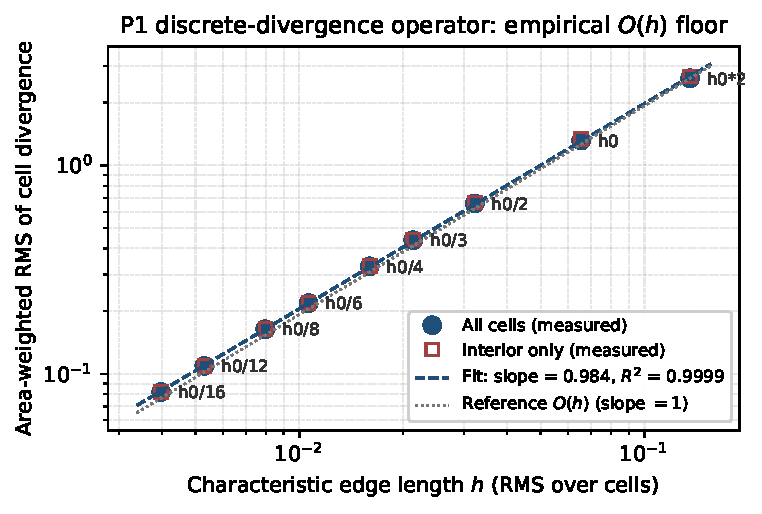
\includegraphics[width=0.82\linewidth]{figures/fig_4_operator_floor_loglog.pdf}
\caption{P1 divergence operator-floor calibration.}
\label{fig:operator-floor}
\end{figure}

\subsection{Fault-detection robustness and coverage boundaries}
\label{subsec:fault-robustness}

To check whether the primary MGN seeded-fault result of Section~\ref{subsec:within-sut-pilot} reproduces beyond one checkpoint and delimit where its detectors are structurally insensitive, the 10-mutant catalogue is replayed against the K=6 multi-checkpoint roster across five input-permutation seeds (30 trials per mutant per detector), with two predeclared severity dimensions swept: \texttt{NS\_double\_scale}, where NS denotes the normalization-scale mutant family and \(s \in \{1.1, 1.25, 1.5, 2, 4\}\), and \texttt{PC\_zero\_vy}, where PC denotes the physical-channel mutant family and the zeroed-\(v_y\) partial fraction is \(p \in \{0.25, 0.5, 0.75, 0.85, 0.9, 0.95, 0.99, 1.0\}\) (the canonical mutant is \(p = 1.0\)). Detection is decided by the same predeclared thresholds as Section~\ref{subsec:within-sut-pilot} (node-permutation tolerance $10^{-5}$, conservation ratio threshold 1.5, mirror-y relative-change threshold 0.5). Wilson 95\% CIs are computed across the (SUT, seed) cells; raw outputs are committed, with claim paths listed in the supplementary evidence appendix. This 10-mutant replay is the primary MGN stress-test denominator, not the whole fault-evidence inventory summarized in Section~\ref{subsec:suts}.

Table~\ref{tab:coverage-geometry} summarizes the coverage geometry that would otherwise be buried in several paragraphs. The table should be read by row: each admitted relation measures one invariant family, and the blind cells are therefore structural, not sampling noise.

\begin{table}[!htbp]
\centering
\caption{Coverage-geometry matrix.}
\label{tab:coverage-geometry}
\scriptsize
\renewcommand{\arraystretch}{0.93}
\begin{tabularx}{\linewidth}{@{}>{\raggedright\arraybackslash}p{0.18\linewidth}>{\raggedright\arraybackslash}p{0.26\linewidth}>{\raggedright\arraybackslash}p{0.26\linewidth}Y@{}}
\toprule
\textbf{Detector / relation family} & \textbf{Visible directions} & \textbf{Blind or excluded directions} & \textbf{Scope and boundary} \\
\midrule
Node permutation & Representation contract passes exactly; also admitted on airfoil & Canonical injected faults preserve node relabeling, so no mutant is detected & Sanity/adapter evidence, not fault-coverage evidence \\
Continuity / conservation & Boundary-condition faults and gross normalization faults; shared continuity $\to$ normalization-scale signal on airfoil & Multiplicative output scaling sweep remains undetected (0/6, CI $[0.00,0.39]$) & Measures conservation-like invariants only; absolute MGN conservation remains deferred \\
Mirror-y symmetry & Physical-channel and mesh-adjacency faults; partial $v_y$ zeroing detected through $p=0.99$ (6/6) & Exactly uniform $p=1.0$ is blind (0/6); mirror-y excluded on non-zero-angle airfoil & Coverage disappears when the relation is inadmissible \\
Admitted suite & 5/10 canonical MGN mutants detected; reproduces across S0--S3, with 4/10 on S4/S5 & Invariant-preserving faults remain invisible, including adversarial escapes & Bounded stress-test coverage, not real-world defect-detection rate \\
Cross-family / cross-program checks & PINN/FNO probes and sibling programs reproduce the invariant-based reading & Trained-mutant MGN/PointMLP evidence and closed-form PINN/FNO probes are not interchangeable & Breadth evidence only; no calibrated coverage law \\
\bottomrule
\end{tabularx}
\end{table}

\textbf{Aggregate reading.} The 5-of-10 union detection rate from the seeded-fault stress test reproduces across S0--S3 and nearly across S4/S5. By-class localization also reproduces: continuity is sensitive to boundary/scale faults, whereas mirror-y is sensitive to physical-channel and adjacency faults. The severity sweeps in Table~\ref{tab:coverage-geometry} delimit the same point: faults are caught when they perturb a measured invariant and are invisible when they preserve all admitted invariants.

\textbf{Unified catalogue and adversarial checks.} Phase 3 emits a 60-entry catalogue (10 canonical MGN mutants, 2 adversarial MGN mutants, 24 closed-form PINN probes, and 24 closed-form FNO probes). Its descriptive precision/recall summary is node-permutation 1.00/1.00, conservation 1.00/0.81, and mirror-y 0.94/0.55; these rates summarize non-independent checkpoint-by-seed cells, not independent population items. The PINN/FNO probes further show a falsifiable blind region: faults preserving every measured invariant are detected by no relation, even when a transport fault corrupts the PINN field by 0.63 relative \(L_2\) norm. \textbf{Adversarial mutants (R4).} Two adversarial MGN mutants test whether the blind region is a subspace, not a point: A1 is detected by mirror-y through magnitude shift, with node-permutation 0/6 and conservation 0/6, so it is not evidence that the node-permutation or conservation detectors cover the blind subspace; A2 escapes every detector.

\textbf{Cross-SUT and cross-program breadth.} On the bounded PhysicsNeMo airfoil task, the gate excludes mirror-y because of non-zero angle of attack, and the mirror-only cylinder-flow coverage disappears; the shared continuity $\to$ normalization-scale signal remains. This supports the qualitative validity-coverage duality, but only at fault-class level on two CFD SUTs. The Minimum-MR-SubSet external-scope audit adds external witness evidence across seven program types and five CPU-only replays; it does not add new primary SUT executions to this paper. The Minimum-MR-SubSet primary rerun records \texttt{PASS\_WITNESS}, kstar = 6, and four active true fault classes on held-out cylinder-flow MGN runtime evidence, not a second architecture or dataset. The Minimum-MR-SubSet PINN primary reruns record \texttt{PASS\_WITNESS}, kstar = 1, and five active true fault classes for Burgers2D and Diffusion2D PINN witnesses; they are one-seed witnesses with no cross-SUT rate. The supplementary evidence appendix gives the details.

\textbf{Independent periodic-advection primary workflow.} The \textbf{periodic-advection primary workflow} adds a new synthetic SciML surrogate task rather than another cylinder, airfoil, PINN, or FNO extension. Six deterministic NumPy-trained periodic-convolution SUTs are trained for one two-dimensional scalar periodic-advection step on a 32 x 32 periodic grid and evaluated on 10 held-out fields per SUT. The run records relation records, trained checkpoints, source/follow-up output archives, per-SUT metric ledgers, gate decisions, and an aggregate verdict report. Periodic integer translation is admitted and gives \textbf{60/60 translation passes} (maximum relative-\(L_2\) violation 0.0 at tolerance $10^{-10}$). Global mass/mean conservation is admitted and gives \textbf{60/60 mass-conservation passes} (maximum root-mean-square (RMS)-normalized mean drift $3.47\times10^{-17}$ at tolerance $10^{-10}$). The \textbf{fixed-velocity mirror candidate is rejected} for 6/6 SUTs and is not executed as an exact MR because mirroring the scalar field without transforming the advection velocity changes the transport problem. This is full gate-to-verdict evidence on an independent primary-scale synthetic PDE task, \textbf{not production CFD or real-defect evidence}.

\textbf{Cross-family PINN extension.} The \textbf{Cross-family PINN extension} is a K=15 roster over Burgers and heat PINNs. MR-A is vacuous by construction for these pointwise PINNs, so the cross-family claim is carried by two non-trivial MR families, MR-B and MR-C. The K=15 roster reports MR-B mean ratios 0.712 on Burgers and 1.495 on heat, with the heat symmetry result mixed; MR-C reports 1.007 on Burgers and 1.006 on heat. This supports predicate transfer to PINN-style outputs without turning the roster into a general PINN reliability or cross-SUT rate.

\subsection{Interpretation and boundaries}
\label{sec:discussion}
\label{subsec:still-blocked}
\label{subsec:scoped-interpretation}

The value of the current study is not that every MR finds a new fault beyond rollout accuracy. Retained MRs provide relation-level evidence under explicit transformations; on a violation or deferral, the relation record and verdict rule help distinguish model inconsistency, relation-domain boundary, numerical tolerance issue, and inconclusive evidence. A detailed interpretation-and-claim-boundary guide is provided in the supplementary evidence appendix.

Two misreadings are especially important. First, without the gate, asymmetric-mesh mirror-y could be read as a model fault rather than an out-of-relation-domain stress result; with the gate, it remains a robustness signal but not a valid-domain defect oracle. Second, without the floor check, absolute discrete-divergence could be misread as a conservation pass despite reference-field divergence. The added runs answer whether this is only post-hoc labeling: the same predicate admits, rejects, or defers relations differently on symmetric meshes, airfoil, PINN, and FNO subjects, while preserving the stated reliability and geometry-independent-rate boundaries.

The canonical blocked list remains active: the evidence does not support external-dataset or geometry-independent pass/fail rates, AeroGraphNet/DoMINO results, comparative superiority over baselines, real-world fault-detection rates, validated localization, runtime, reliability, or model accuracy claims. The supported claim is that an admissibility-gated workflow makes MR identification and execution more auditable for the studied class of SciML SUTs.

The scoped evidence shows how SciML testing can move from implicit expert checks to explicit relation records and executable checks that complement residuals, UQ, and accuracy by making transformations and verdict rules inspectable. The workflow targets a relation-indexed applicability map in relation space rather than residual space; calibrated maps across SUTs, trajectories, and domain-violation scores remain future work.

The gate earns its overhead when a surrogate must be trusted out of distribution and a physically necessary relation can be both stated for the task and made numerically decidable for the deployed discretization. Authoring an admissible MR requires domain knowledge to state the relation, numerical analysis to set or reject the floor, and testing expertise to bind transformations, mappings, metrics, and ledger fields. The workflow decomposes those roles and provides reusable records and runners, but it does not measure person-hours, inter-author agreement, or maintenance cost; those are adoption questions for future work.

\section{Threats to Validity}
\label{sec:threats}

We classify threats following Verdecchia et al.~\citep{verdecchia2023threats} and report against the Empirical Standards for software engineering research~\citep{ralph2021empirical}.

\textbf{Ethics and evidence integrity.} The study does not involve human subjects or personal data. SUT versions, datasets, checkpoints, scripts, and run logs are recorded when licensing permits, and failed, skipped, out-of-relation-domain, numerical-tolerance, and inconclusive outcomes remain in the evidence records. LLM use is restricted to candidate generation and evidence organization, not validity judgment. No candidate MR is described as valid without a passing gate decision and relation record; no OOD violation is described as a program fault without supporting verdict evidence.

\textbf{Construct validity.} The main construct is not ``model correctness'' but admissibility-gated MR checking. A wrong physical premise, boundary-condition reading, output mapping, discrete operator, or tolerance could therefore change an admit/reject/defer decision. We mitigate this by requiring a relation record, explicit preconditions, typed verdicts, and an operator-floor argument before a relation is treated as executable evidence. The mitigation is still incomplete: the P1 divergence floor is derived for the deployed symmetric-mesh setting and is empirically stable on a second unstructured Delaunay topology but is not proven for arbitrary unstructured meshes, and the reference-relative conservation diagnostic remains a non-regression guard rather than an absolute conservation measurement. The seeded-fault catalogue also measures detector sensitivity to author-implemented mutants, so its rates do not estimate real-world defect prevalence or effectiveness. A gate verdict can prevent invalid fault attribution, but it must not be read as dismissing deployment robustness concerns outside the relation domain.

\textbf{Internal validity.} SUT setup, checkpoint selection, random seeds, mesh preprocessing, normalization, and runtime nondeterminism may affect verdicts. The study records manifests, ledgers, and raw outputs, and it repeats the primary cylinder-flow checks across K=6 checkpoints, three held-out trajectories, same-task variants, PointMLP, and PhysicsNeMo. These repetitions reduce the risk of a single-run artifact, but do not make the cells independent population samples. For airfoil, high one-step rollout error is read as training-state context, not model accuracy evidence.

\textbf{External validity.} The evidence covers incompressible cylinder flow, compressible airfoil flow, bounded PINN/FNO Burgers and heat executions, an independent periodic-advection primary workflow over six synthetic periodic-convolution SUTs, and a read-only/executed cross-program breadth check from the Minimum-MR-SubSet sibling artifacts. These cases make the gate less likely to be a one-off cylinder-flow checklist, but they remain far from a general claim about SciML surrogates. The periodic-advection run adds a complete gate-to-verdict chain on a different PDE/operator setting; it does not convert the evidence into production CFD, real-defect, or reliability rates. Broader neural operators, mesh simulators, production CFD solvers, PINN architectures, datasets, geometries, and training regimes remain outside the evidence. The cross-program breadth check reuses the sibling's domain evidence and mutant sets, so it supports only a qualitative coverage-geometry reading, not per-program reliability, new MR discovery, superiority, or real-world fault-detection rates.

\textbf{Baseline and comparator validity.} Rollout accuracy, residual/UQ-style diagnostics, generic MR templates, and LLM-assisted candidate generation are used as scope contrasts rather than defeated competitors. The LLM baselines depend on prompt design, model versions, and simulated raters; they show why an admissibility gate is needed, but are not a human-expert study and do not establish superiority over alternative MR-identification methods. The deterministic admissibility gate, not LLM output, is the validity authority.

\textbf{Conclusion validity.} The study combines descriptive counts, Wilson intervals, bootstrap intervals, and exact nonparametric tests where the sampling unit supports them. Many reported cells share checkpoints, trajectories, or generated cases, so are not independent population trials. The primary MGN scope upgrade improves the weakest denominators within the stated scope, but the correct conclusion is bounded empirical utility for RQ4, not a calibrated reliability or coverage rate.

\textbf{Reproducibility.} Some workflows depend on old runtimes, public benchmark loaders, or non-redistributable checkpoints. The replication package therefore emphasizes scripts, manifests, run logs, claim ledgers, and available outputs. Reproducibility is strongest for artifact inspection and rerunnable CPU workflows, weaker for exact recreation of every trained checkpoint environment. By re-run cost: the operator-floor sweep, relation-record validators, and typed-verdict logic replay on CPU in minutes from committed scripts alone; the cylinder-flow MGN pilot, K=6 roster, PointMLP, and FNO/PINN rosters replay on CPU from committed checkpoints and metric ledgers; PhysicsNeMo MGN and airfoil training require a graphics-processing unit (GPU) and the public DeepMind TFRecords; and the Minimum-MR-SubSet audit and rerun execute read-only from sibling fixtures at the cited commit.

\section{Future Work}
\label{sec:future-work}

Future work should generalize the numerical-decidability theory beyond shape-regular P1 triangular settings to degenerate/sliver-heavy meshes, boundary treatments, flux-form operators, discontinuous fields, and learned-output-specific floor models. The present evidence supports a local shape-regular P1 bound, a tighter closed-form and bounded floor for the concrete structured setting, and observed stability on one Delaunay topology; it does not provide an arbitrary-mesh theorem.

Second, the domain-violation axis should be calibrated across MR families. Here, domain distance is a per-relation interpretive coordinate, not a cross-MR score. A calibration protocol would normalize distances within relation families, define in-domain/near-boundary/out-of-relation-domain anchor cases, build relation-family calibration sets, and use independent experts or raters to validate categories, agreement, and residual comparability limits.

Third, the relation-record workflow should be evaluated on production-scale SUTs and datasets: external aerodynamics, production graph simulators, longer rollouts, and multi-physics pipelines.

Fourth, the coverage implication should be tested with independent real-defect corpora and independently authored mutants, asking whether admitted MR sets predict externally collected defect classes.

Finally, relation-record authoring, precondition checking, and ledger generation need automation and user studies of authoring effort, role division, inter-author agreement, and maintenance cost, while validity decisions remain tied to physical, numerical, and software evidence rather than model consensus.

\section{Conclusion}
\label{sec:conclusion}

The central question was when a physics-derived MR for SciML surrogate software is sound enough to use as an oracle-free test. The answer is a numerical-decidability admissibility criterion embedded in an admissibility-gated workflow: a candidate relation is first checked for physical basis, domain preconditions, representation mapping, and numerical decidability; admitted relations are recorded as relation records and executable checks; and outcomes are interpreted with typed verdicts rather than a single pass/fail label.

The empirical evidence is bounded but artifact-backed. On cylinder-flow MeshGraphNets, the workflow separates a representation pass, an out-of-relation-domain mirror probe, a deferred absolute conservation relation, and a reference-relative diagnostic. The operator-floor analysis shows why the conservation verdict is not numerically decidable as an absolute test in that setting, while alternative settings admit executable conservation checks. On airfoil, PINN, FNO, and cross-program subjects, the gate changes or preserves verdicts according to the relation's physical and numerical conditions. Seeded-fault stress tests further show that the admitted MR set helps explain detector blind spots in the studied settings, without implying general defect-detection rates or excusing OOD robustness failures.

The contribution is therefore methodological and evidentially bounded: physically meaningful SciML metamorphic tests require explicit validity conditions, a numerically decidable verdict, executable checks, raw evidence records, and relation-level verdicts. This turns candidate MRs from informal expert intuitions into auditable tests with boundaries visible to reviewers and practitioners, while leaving arbitrary-mesh theory and general defect-rate evaluation as open work.

\section*{Preprint}
An earlier preprint version of this manuscript is available on arXiv at \url{https://arxiv.org/abs/2606.17529} with DOI \url{https://doi.org/10.48550/arXiv.2606.17529}.

\section*{CRediT authorship contribution statement}
\textbf{Meng Li:} Conceptualization, Methodology, Software, Writing -- original draft. \textbf{Xiaohua Yang:} Supervision, Formal analysis, Writing -- review \& editing. \textbf{Jie Liu:} Investigation, Validation. \textbf{Shiyu Yan:} Data curation, Visualization.

\section*{Declaration of competing interest}
The authors declare no conflict of interest.

\section*{Declaration of generative AI and AI-assisted technologies in the writing process}
During the preparation of this work the authors used generative AI assistants for code scaffolding, prose copy-editing, and reference cross-checking. After using these tools the authors reviewed and edited the content as needed and take full responsibility for the content of the publication. No generative AI was used to fabricate, alter, or invent experimental data, results, or citations; every numerical claim is backed by a tracked artifact under \texttt{research\_assets/runs/} and a claim-ledger entry.

\section*{Acknowledgments}
This work was supported by the National Natural Science Foundation of China (NSFC) General Program (grant no.\ 12575176), the Hunan Provincial Education Department Project, China (grant no.\ 202502000728), the Natural Science Foundation of Hunan Province, China (grant no.\ 2025JJ70193), and an industry-funded research project (grant no.\ 230KHX060001).

\section*{Data availability}
The replication package is archived on Zenodo at \url{https://doi.org/10.5281/zenodo.20702952}, with source at \url{https://github.com/meng004/Domain-Validity-Gated-MR-for-SciML}. It contains the manuscript source, relation records, validators, claim ledger, run manifests, metric ledgers, and committed derived outputs under \path{research_assets/runs/}. Minimum-MR-SubSet audit/rerun artifacts cite commit \path{9ef862ec37335b4834d0a1fb38b4b613af702f34}. DeepMind cylinder-flow and airfoil TFRecords are public benchmark inputs staged by the workflow runners rather than redistributed in the manuscript package. GPU-dependent reruns and credential requirements are documented in \path{REPRODUCIBILITY.md}; absent credentials cause fail-closed precondition checks rather than silent substitution.

\bibliographystyle{elsarticle-num}
\bibliography{references}

\end{document}
